\section{Results}
Table~\ref{tab:rq} shows the verdict for every prespecified criterion. Most criteria were met: five of the nine questions were supported, and the two descriptive questions (same-protocol comparison and components) were answered. Detection was partly supported because one of the four external cohorts was below the 0.70 threshold, and the slow-wave grade missed its criterion by only 0.007.

\begin{table*}[!t]
\caption{Prespecified research questions, criteria and verdicts (computed mechanically by the analysis code).}
\label{tab:rq}
\centering
\scriptsize
\begin{tabular}{@{}p{1.75cm}p{7.1cm}p{6.9cm}p{1.7cm}@{}}
\toprule
Question & Criterion (abridged) & Observed & Verdict \\
\midrule
Detection & Pooled F1 $\geq$ 0.75 and precision--recall area $\geq$ 0.85; full support needs F1 $\geq$ 0.70 in every cohort & F1 0.849, area 0.933; external F1 0.866 (ISRUC-II), 0.869 (ISRUC-III), 0.704 (DOD-H), 0.580 (DOD-O) & Partially supported \\ % research_question_results.csv
Same-protocol & Same-protocol comparison with four published models, paired, Holm-corrected & see Table~\ref{tab:sota} & Answered \\
Factor validity & Signal factors and continuity higher early than late in the night and for expert N3 than N2; full support needs the rating to rise with the fraction of experts voting N3 & all four factors higher early and for N3; graded agreement median $\rho$ = 0.81 & Supported \\
Grade & Slow-wave coverage separates expert stage 4 from stage 3 (CAP) with area $\geq$ 0.75; High share higher early; grade rises with expert vote & area 0.743; early $>$ late $p = 1.9\times10^{-22}$; $\rho$ = 0.318 & Not supported \\
Stability & 5th-percentile Spearman $\rho \geq$ 0.90 under weight perturbation; early $>$ late within each training cohort & $\rho$ = 0.979; HMC $p = 3.1\times10^{-13}$, ISRUC-I $p = 3.6\times10^{-8}$ & Supported \\
Components & Component effects on identical folds, paired, Holm-corrected & see Table~SII & Answered \\
Explanations & Delta top band for perturbation and integrated gradients in $\geq$ 70\% of participants; surrogate top group delta with fidelity $R^2 \geq$ 0.70 & 100\% and 100\% of participants; $R^2$ = 0.86 & Supported \\
Reliability & Error-detection area $\geq$ 0.75 and F1 at 80\% coverage above F1 at 100\% & area 0.879; F1 0.949 vs 0.849 & Supported \\
Profile & Predicted vs expert N3 minutes per night, ICC(2,1) $\geq$ 0.75 & ICC 0.806 & Supported \\
\bottomrule
\end{tabular}
\end{table*}

\subsection{N3 detection}
The detector achieved high accuracy: across the 251 cross-validation participants, it reached an F1 score of 0.849 (95\% CI 0.838--0.861) and a precision--recall area of 0.933 (Table~\ref{tab:detection}, Fig.~S1). Performance was similar in the two training cohorts and remained high in ISRUC-II, ISRUC-III and CAP (F1 0.831--0.869). In DOD-H and DOD-O, the ranking of epochs was still excellent (ROC area 0.990 and 0.984), but precision dropped to 0.545 and 0.409 at a recall of 0.994 and 0.996. The detector labelled many consensus N2 epochs as N3 (Fig.~\ref{fig:cm}). DOD-O did not reach the 0.70 threshold, so detection is only partly supported. % rq1_detection_metrics.csv

\begin{table}[!t]
\caption{N3 detection. Cross-validation (CV) values are out-of-fold; external cohorts are predicted by the five-fold ensemble. 95\% participant-level bootstrap intervals.}
\label{tab:detection}
\centering
\setlength{\tabcolsep}{2.5pt}
\footnotesize
\begin{tabular}{@{}lrcccc@{}}
\toprule
Set & $n$ & F1 (95\% CI) & PR area & ROC area & $\kappa$ \\
\midrule
CV pooled & 251 & 0.849 (0.838--0.861) & 0.933 & 0.978 & 0.812 \\ % rq1_detection_metrics pooled_all_cohorts
CV HMC & 151 & 0.832 (0.813--0.848) & 0.921 & 0.973 & 0.790 \\
CV ISRUC-I & 100 & 0.877 (0.863--0.890) & 0.950 & 0.985 & 0.847 \\
\midrule
ISRUC-II & 8 & 0.866 (0.791--0.905) & 0.905 & 0.983 & 0.834 \\
ISRUC-III & 10 & 0.869 (0.847--0.890) & 0.968 & 0.990 & 0.835 \\
CAP & 105 & 0.831 (0.810--0.848) & 0.919 & 0.962 & 0.780 \\
DOD-H & 25 & 0.704 (0.651--0.749) & 0.946 & 0.990 & 0.639 \\
DOD-O & 55 & 0.580 (0.525--0.631) & 0.883 & 0.984 & 0.506 \\
\bottomrule
\end{tabular}
\end{table}

\begin{figure}[!h]
\centering
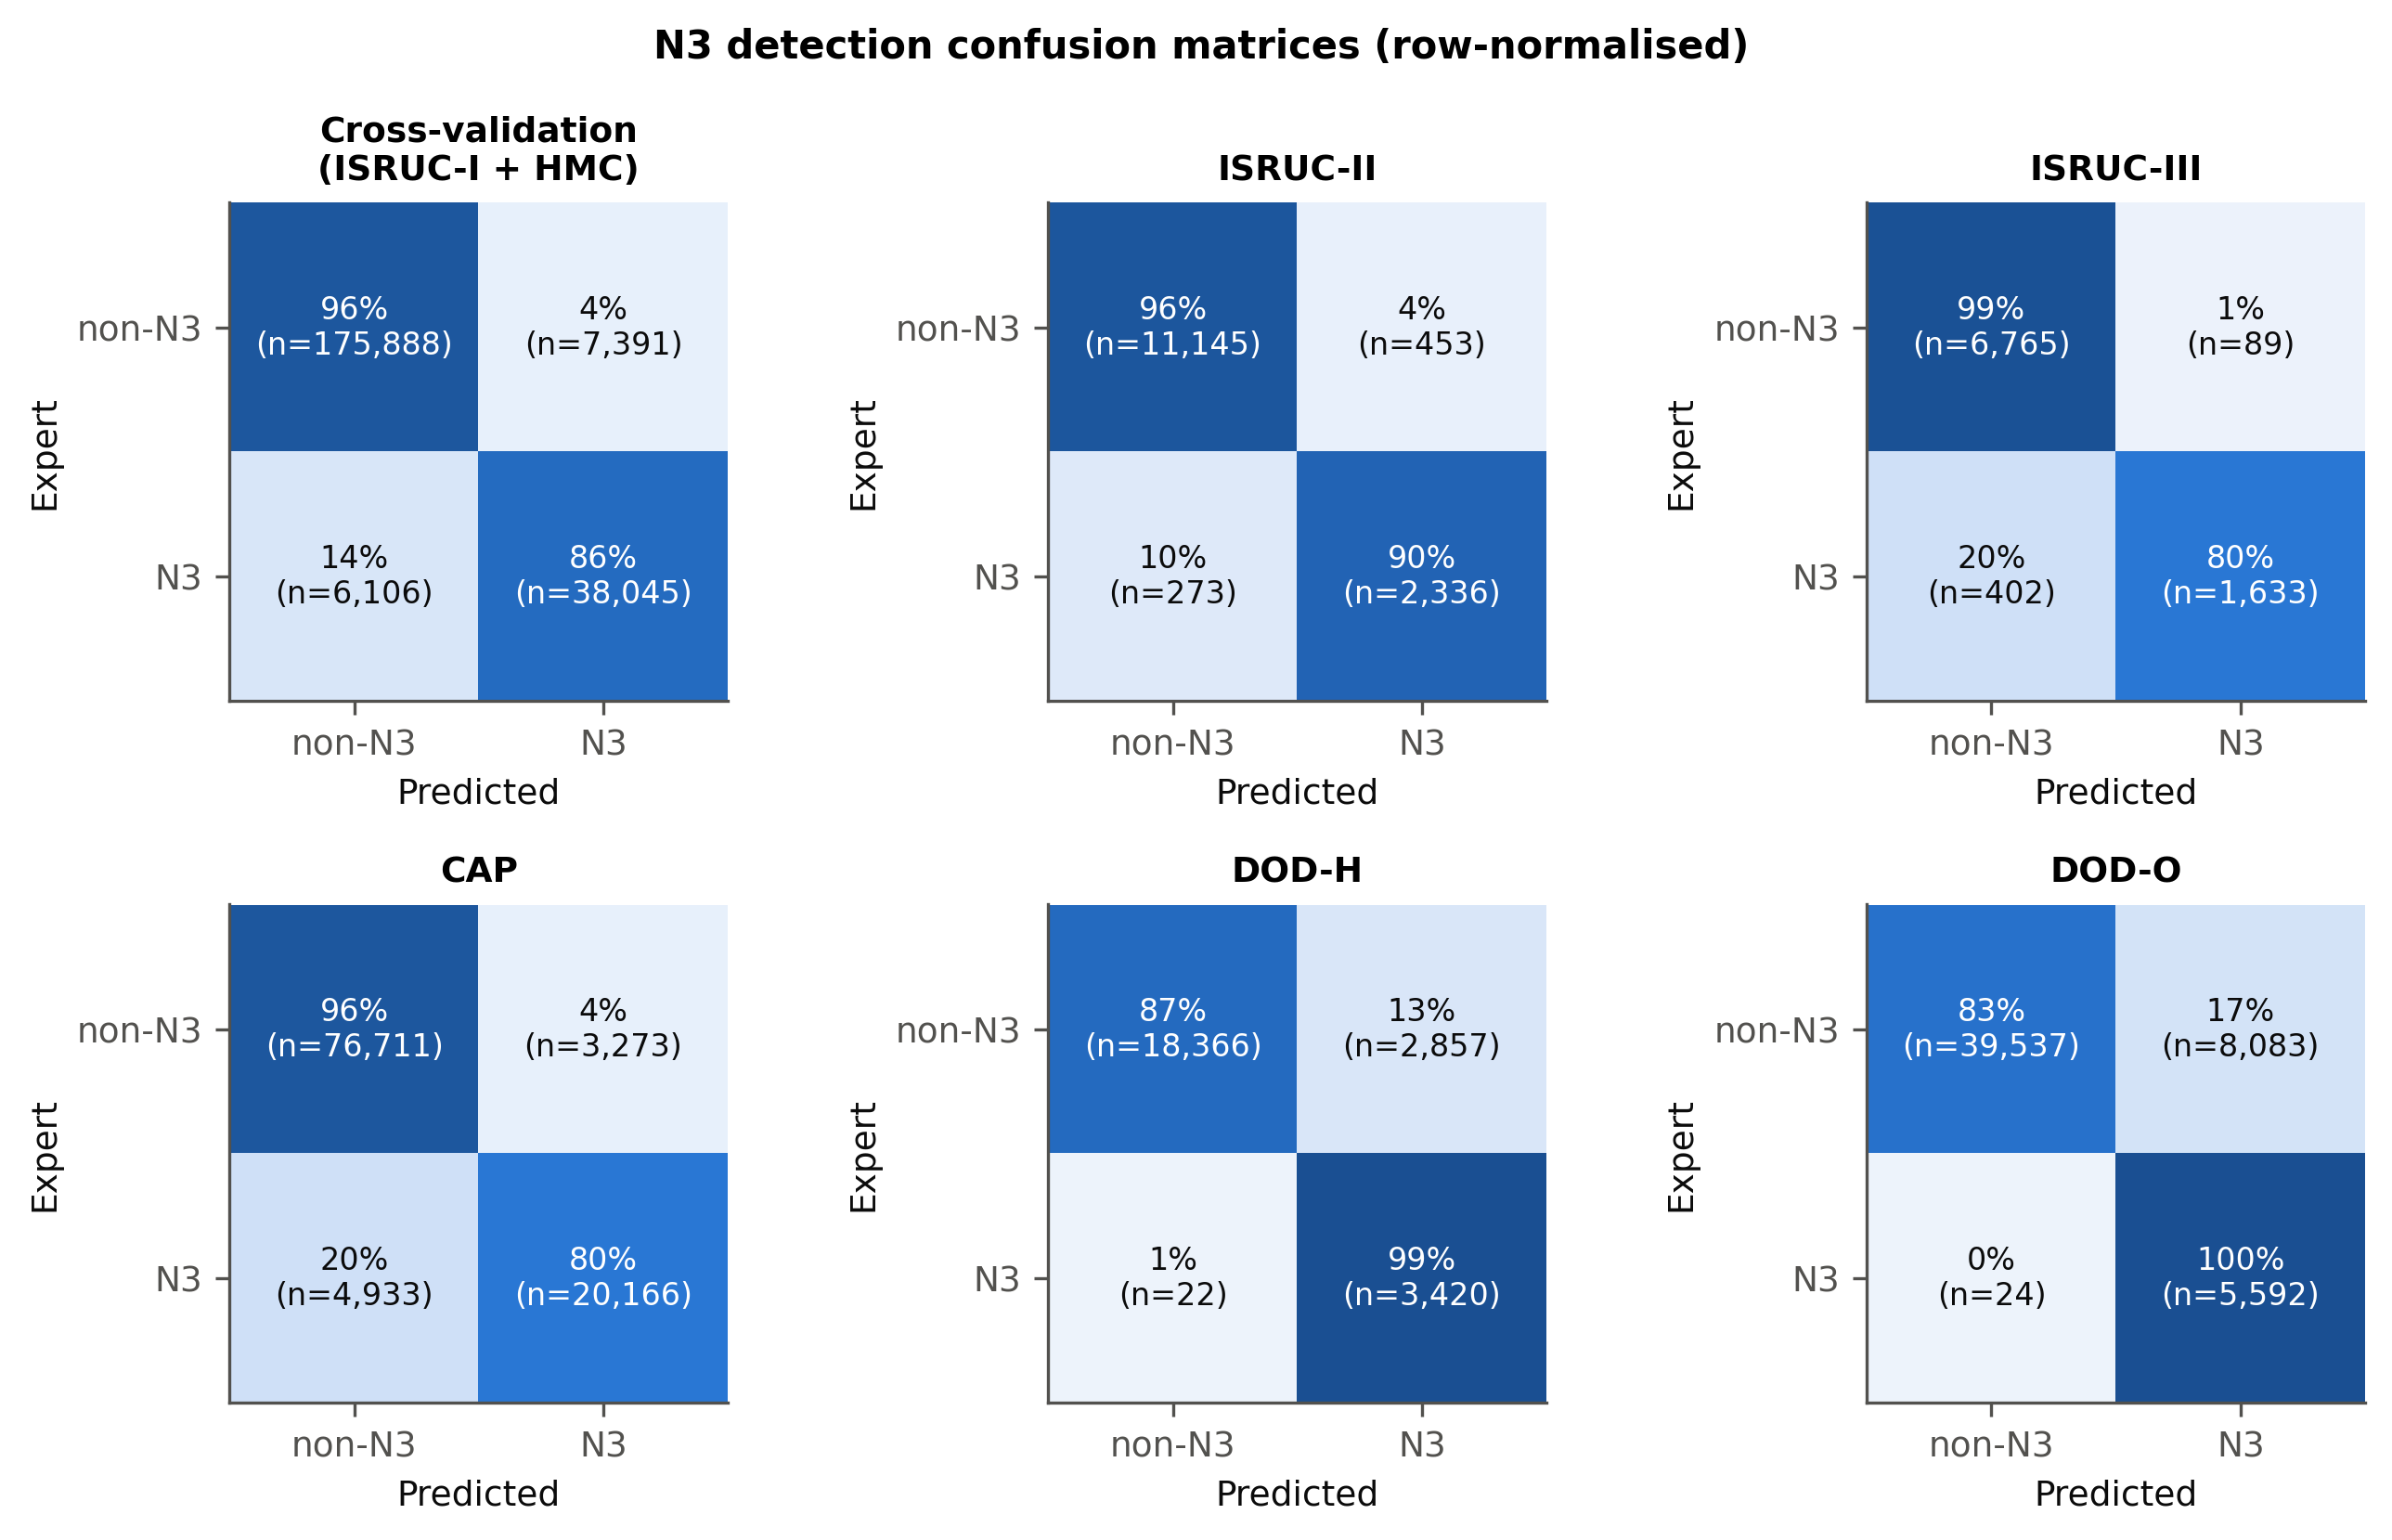
\includegraphics[width=0.5\columnwidth]{fig_rq1_confusion_matrices.png}
\caption{Row-normalised confusion matrices for N3 versus non-N3 epochs (counts in brackets). DOD cohorts show near-complete recall with more false positives; 96\% of these were scored N2 by the consensus.}
\label{fig:cm}
\end{figure}

% fig caption 96%: sensitivity_rq1_false_positive_structure.csv fp_expert_N2 DOD-H 0.966, DOD-O 0.964

The false positives in DOD did not occur at random. Of the DOD-O false positives, 96.4\% were consensus N2 epochs and 60.9\% had at least one of the five experts voting N3; in DOD-H the figures were 96.6\% and 51.0\%. In a post hoc analysis with a lenient reference (N3 if any expert scored N3), F1 rose to 0.834 in DOD-H and 0.819 in DOD-O; on epochs on which all experts agreed it was 0.740 and 0.550. Leave-one-cohort-out models reached DOD F1 scores between 0.624 and 0.739, so the drop is not caused by the ensemble. After temperature scaling, the expected calibration error was 0.022--0.061 in cross-validation, ISRUC and CAP, but 0.192 (DOD-H) and 0.225 (DOD-O) (Fig.~S2). % sensitivity_rq1_false_positive_structure; sensitivity_matrix; rq1_detection_metrics LOCO rows; ledger_extra ECE

\textit{Comparison with human scorers.} In ISRUC-I and ISRUC-II, the model agreed with single experts more closely than the experts agreed with each other (mean F1 0.867 vs 0.849 and 0.883 vs 0.861); this was true for each scorer separately (lowest model--scorer F1 0.858 and 0.866), although in ISRUC-I the model was trained, out of fold, on labels of the first scorer from the same centre. In DOD-O, where experts agreed least (mean pairwise F1 0.603, range 0.494--0.701), model--expert agreement (0.588, range 0.485--0.762) was inside the expert range. In DOD-H (0.695 vs 0.772, expert range 0.708--0.806) and ISRUC-III (0.881 vs 0.917), it was lower. % rq1_interrater_benchmark.csv


\subsection{Same-protocol comparison}
Table~\ref{tab:sota} shows the four published architectures trained under the same protocol. The proposed detector and DeepSleepNet did not differ significantly (median participant difference in F1 +0.005, Holm $p$ = 0.15; Fig.~S3), although DeepSleepNet has 264 times more parameters and needed 36.2 instead of 1.6 minutes per fold (wall-clock times on shared cloud GPUs, indicative only). The detector outperformed TinySleepNet (+0.011, $p$ = 0.0032), L-SeqSleepNet (+0.021, $p = 1.6\times10^{-8}$) and AttnSleep (+0.031, $p = 9.5\times10^{-18}$). Among the five same-protocol models, it had the highest external F1 score in ISRUC-II, DOD-H and DOD-O (0.866, 0.704, 0.580); DeepSleepNet was highest in CAP (0.836 against 0.831), and TinySleepNet and L-SeqSleepNet in ISRUC-III (0.903 against 0.869); all external values are in the repository. The pretrained open stager YASA, applied without any change, reached F1 scores of 0.79 in the training cohorts, 0.60--0.77 in ISRUC-II, ISRUC-III and CAP, and 0.79 and 0.72 in DOD-H and DOD-O; like the proposed detector, its precision dropped in DOD (0.66 and 0.57, compared with 0.87--1.00 elsewhere) while recall rose to 0.97. Its five-class decision is more cautious than our F1-optimised threshold, so the precision--recall area gives a fairer comparison: 0.907, 0.893, 0.910, 0.885, 0.962 and 0.864 in the training cohorts, CAP, DOD-H, DOD-O, ISRUC-III and ISRUC-II, compared with 0.933, 0.919, 0.946, 0.883, 0.968 and 0.905 for the proposed detector, on the same epochs in every cohort. % posthoc3_isruc2_same_nights.csv % posthoc2_yasa_comparator.csv % rq1_sota_comparison.csv, rq1_sota_paired_tests.csv

\begin{table}[!t]
\caption{Same-protocol comparison: cross-validation F1 (95\% CI), PR area, parameters and training time per fold. $\Delta$F1: median paired participant difference (proposed minus baseline) with Holm-corrected $p$.}
\label{tab:sota}
\centering
\setlength{\tabcolsep}{2pt}
\footnotesize
\begin{tabular}{@{}lccrrr@{}}
\toprule
Model & CV F1 & PR area & Params & min & $\Delta$F1 ($p$) \\
\midrule
Proposed & 0.849 (0.838--0.861) & 0.933 & 96k & 1.6 & -- \\ % rq1_sota_comparison
DeepSleepNet & 0.846 (0.835--0.857) & 0.925 & 25.4M & 36.2 & +0.005 (0.15) \\
TinySleepNet & 0.841 (0.829--0.852) & 0.925 & 1.5M & 4.5 & +0.011 (0.0032) \\
AttnSleep & 0.817 (0.803--0.829) & 0.904 & 513k & 36.1 & +0.031 ($<$0.001) \\
L-SeqSleepNet & 0.826 (0.812--0.839) & 0.907 & 208k & 4.7 & +0.021 ($<$0.001) \\
\bottomrule
\end{tabular}
\end{table}

\subsection{Validity of the factor scores}
In detected N3 of the training cohorts, delta intensity was 8.8 points higher in the first than in the second half of the night (95\% CI 6.8--10.8, $n$ = 213 participants), slow-wave morphology 9.0 (7.0--11.4), spectral dominance 4.5 (2.8--7.5) and the rating 7.2 (5.4--8.9); all $p < 10^{-5}$ (Fig.~S4). Continuity was also higher early in the night ($p = 3.3\times10^{-6}$), but its median difference was zero because most N3 epochs have only N3 neighbours. Expert N3 epochs scored higher than expert N2 epochs on every factor (median differences 30.8--37.8 points for the three signal factors, 249 participants; Fig.~S5). For delta intensity, morphology and the rating, the decline was repeated in all five external cohorts, and in CAP it was found for every factor. % rq2_factor_validity.csv

The scores also followed the graded judgement of human experts (Fig.~\ref{fig:graded}). On epochs that every expert scored as N2 or N3, each score increased with the fraction of experts who chose N3. The median within-participant Spearman correlation across 198 participants was 0.74 for delta intensity, 0.76 for morphology, 0.75 for spectral dominance and 0.81 for the rating, and it ranged from 0.79 to 0.81 for the rating in every cohort. Without the detector-derived continuity factor, the signal-only composite reached 0.76. When only detected N3 epochs were used, which tests the within-N3 claim directly, the correlations were lower but still positive in every cohort (rating median 0.56, from 0.26 in ISRUC-III to 0.80 in DOD-H; composite 0.53); in ISRUC, with two scorers, the expert fraction has only three levels. The signal factors are calculated from the EEG alone (expert labels are used only for the percentile scale of the training fold, a monotone transform that does not change a Spearman correlation). This agreement therefore shows convergent validity with the visual feature that experts score, not an independent physiological reference. Morphology and the grade use the same amplitude-and-coverage definition that experts apply, so part of this agreement follows from the definition. % rq2_factor_validity.csv graded rows

\begin{figure*}[!t]
\centering
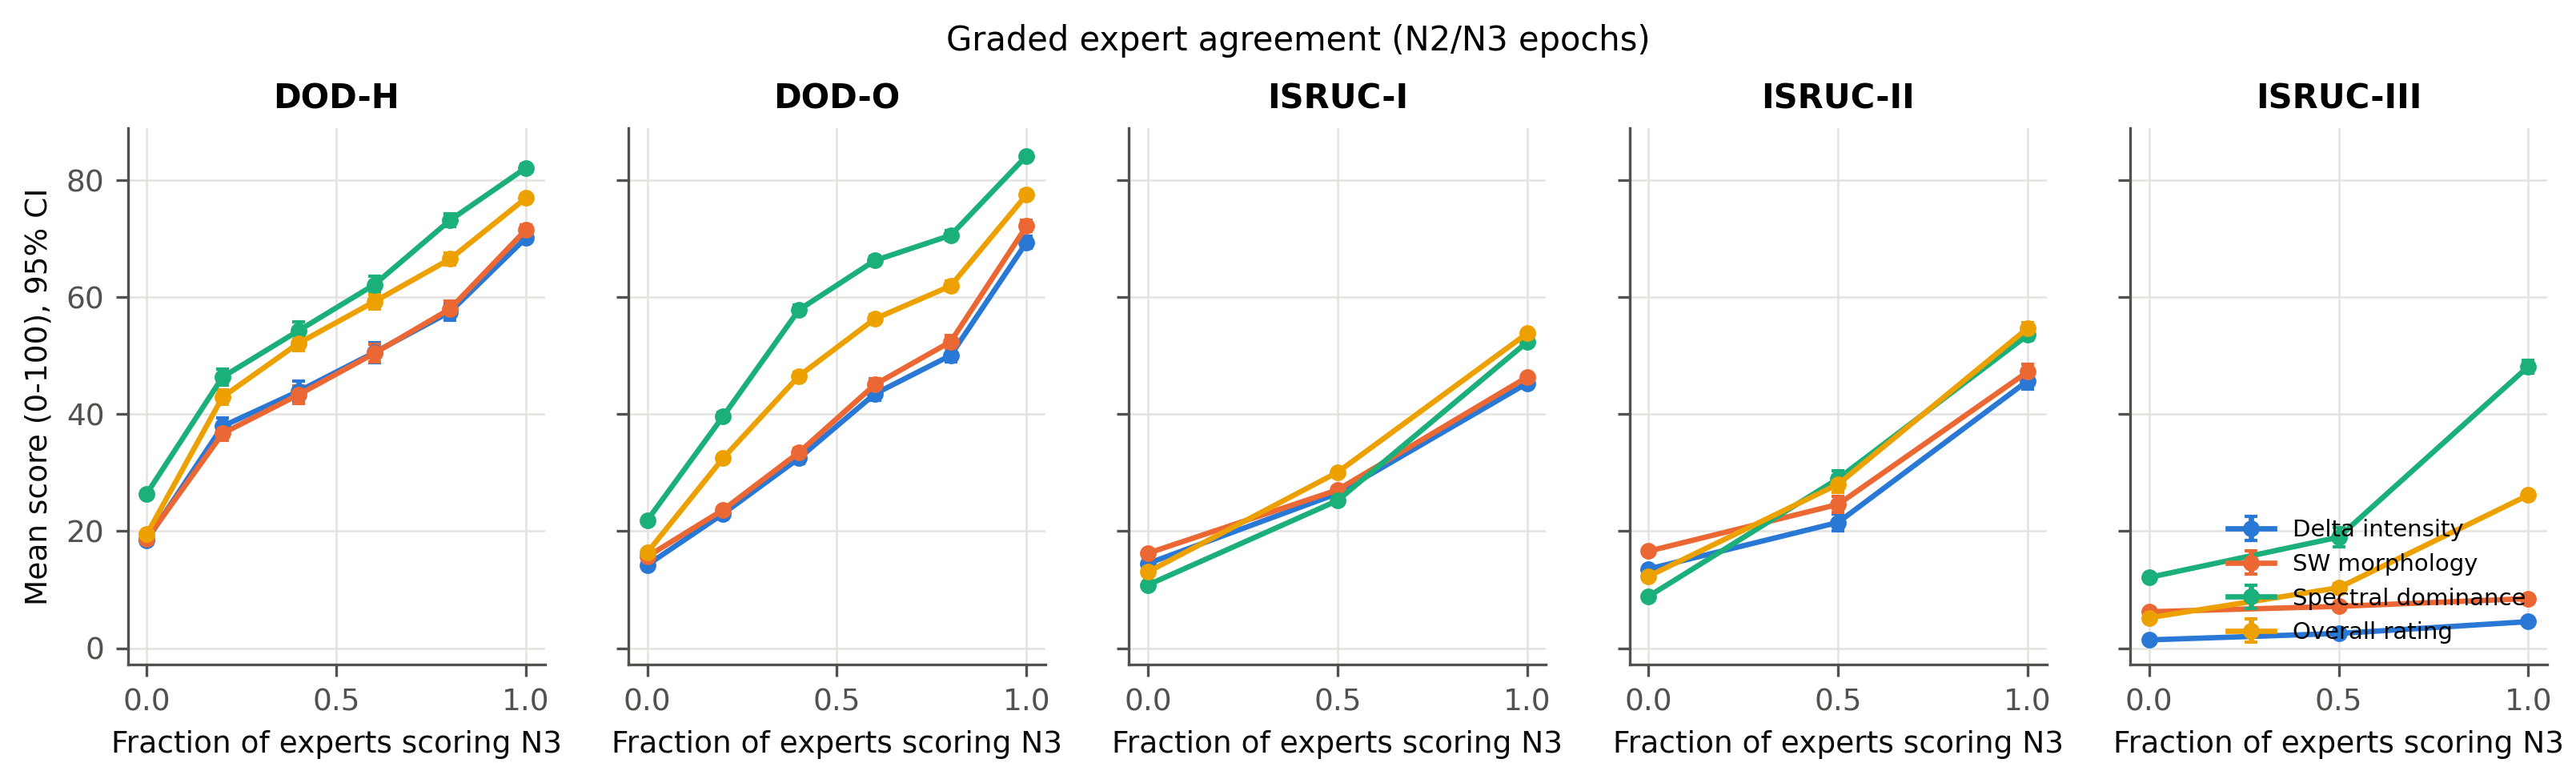
\includegraphics[width=0.56\textwidth]{fig_rq2_graded_expert_agreement.png}
\caption{Graded expert agreement. Mean factor scores and rating (95\% CI) by the fraction of experts who scored an epoch as N3, restricted to epochs scored N2 or N3 by every expert. DOD: five experts; ISRUC: two experts. The low absolute level of the amplitude-dependent scores in ISRUC-III is discussed in Section~\ref{sec:limitations}.}
\label{fig:graded}
\end{figure*}

\subsection{Within-N3 slow-wave grade}
In CAP, slow-wave coverage separated expert stage 4 from stage 3 epochs with an area of 0.782 over all stage 3/4 epochs and 0.743 over epochs that the detector also labelled N3. The prespecified criterion (0.75 on detected epochs) was therefore missed by 0.007. Within participants, the median area was 0.811. The grade was cautious: 98.7\% of stage 3 epochs were not graded High, but only 21.1\% of stage 4 epochs were graded High (Cohen's $\kappa$ 0.15; grade shares in Table~SIII). The High share was larger early in the night ($p = 1.9\times10^{-22}$), the grade rose with the expert vote (epoch-level $\rho$ = 0.318), and the High share was stable across the two ISRUC-II nights (ICC 0.988, $n$ = 8). The thresholds come from both scoring systems and the validation reference is scored with Rechtschaffen and Kales rules, so this shows agreement with R\&K stage 3/4 rather than with AASM N3 grading. % rq2_rk_grade_validation.csv, rq2_n3_grade_validity.csv, sensitivity_rq2b.csv


\subsection{Stability of the rating}
Under random Dirichlet perturbation of the weights around the prior, the 5th-percentile Spearman correlation with the prior-weighted rating was 0.979. Equal weights and weights from the first principal component gave correlations of 0.989 and 0.998, and dropping any single factor kept the correlation between 0.977 and 0.992. In the eight ISRUC-II participants recorded twice, the median nightly rating had a test--retest ICC of 0.763 (95\% CI 0.23--0.95), compared with 0.658 (0.01--0.92) for predicted N3 minutes and $-$0.008 ($-$0.63 to 0.65) for expert-scored N3 minutes. Delta intensity and morphology were similar (Fig.~S6, Table~SIV); spectral dominance was not stable (0.339). With only eight participants the intervals overlap, so this comparison is descriptive. % rq3_overall_rating_stability.json, rq7_profile_agreement.csv test-retest rows

\subsection{Component contributions}
The temporal-context block gave the largest gain (F1 +0.023, 95\% CI 0.018--0.027, Holm $p = 7.3\times10^{-16}$), and the convolutional backbone outperformed a features-only gradient-boosting model by 0.036 (Table~SII). Without the context block, none of the other components changed F1 significantly. Three training seeds of the full model gave F1 scores of 0.849, 0.844 and 0.844 (standard deviation 0.003), so differences below about 0.005 should not be interpreted. In the post hoc leave-one-component-out analysis from the full model, removing feature fusion lowered F1 by 0.0071 (95\% CI 0.0030--0.0108, Holm $p$ = 0.018), an effect larger than the largest seed-to-seed difference (0.0042; Fig.~S7). Removing class weighting or attention, shortening the context to $\pm$3 epochs, or restricting the features to the ten delta-related ones did not change F1 more than seed variability. % rq4_component_effects.csv, rq4_seed_variability.csv, rq4_extended_component_effects.csv



\subsection{Explanations}
Removing the delta band reduced the N3 probability by a median of 0.456, against 0.0005 for the alpha band, and delta was the top band for both perturbation and integrated gradients in all 600 epochs (one to five per participant). The rank correlation between the two methods across bands was 0.7, and the Shapley surrogate (fidelity $R^2$ = 0.86) also ranked the delta feature group first. The same delta dominance held for false positives, false negatives and external cohorts (Fig.~S8). Because N3 is defined by delta waves and delta features are among the inputs, this dominance is expected and is a consistency check rather than evidence that the network learned slow waves. Attention weights correlated weakly and negatively with slow-wave locations (median $\rho = -0.13$), so we do not use attention as an explanation. % rq5_summary.json, rq5x_band_importance_by_outcome.csv

\subsection{Reliability}
The cross-fitted reliability score found misclassified epochs with an area of 0.879 (Fig.~S9). Excluding the 20\% least reliable epochs raised F1 from 0.849 on all epochs to 0.949 on the remaining 80\%, while keeping 72\% of expert N3 and 64\% of expert N2 epochs, and the error rate was 0.9\% in the high, 13.1\% in the medium and 24.6\% in the low category. Most of the signal came from model confidence (0.872) and the Mahalanobis distance (0.855; Table~SV); the quality-control flags alone did not detect errors (areas 0.30--0.48). The score also identified epochs on which the two ISRUC-I experts disagreed (area 0.883). Externally, the area was 0.853 in CAP, 0.872 in ISRUC-II and 0.941 in ISRUC-III but 0.751 in DOD-H and 0.689 in DOD-O, where confidence alone reached 0.683 and 0.612. % rq6_reliability_components.csv, rq6_reliability_categories.csv, rq6_risk_coverage.csv, sensitivity_rq6.csv


\subsection{Episodes and overnight profile}
\begin{figure}[!t]
\centering
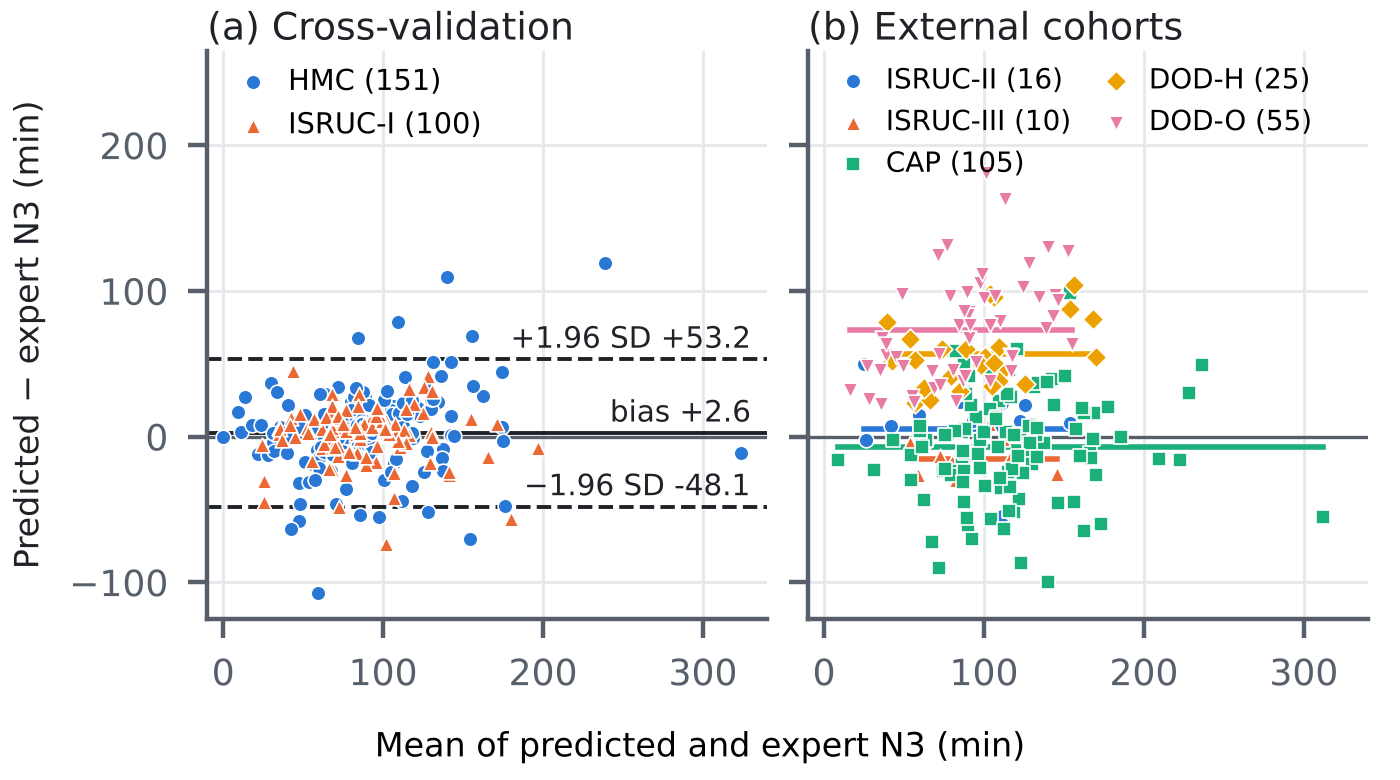
\includegraphics[width=0.86\columnwidth]{fig_rq7_bland_altman_main.png}
\caption{Bland--Altman plots of nightly N3 minutes, predicted minus expert. (a) Cross-validation with bias and 95\% limits of agreement. (b) External cohorts; horizontal lines show each cohort's mean difference. Numbers in brackets are recordings (ISRUC-II: two nights of eight participants).}
\label{fig:ba}
\end{figure}

Predicted and expert N3 minutes per night agreed with ICC 0.806 (95\% CI 0.758--0.845) in cross-validation (bias +2.6 min, limits $-$48.1 to 53.2 min; Fig.~\ref{fig:ba}a). The share of N3 in the first half of the night (0.929), the longest episode (0.780) and the median rating (0.950) also agreed; the episode count (0.622) and median episode duration (0.431) agreed less and are treated as exploratory. Externally, N3 minutes agreed in ISRUC-II (0.898 and 0.740 for the first and second night, eight participants each), ISRUC-III (0.794) and CAP (0.730), but not in DOD-H (0.403) or DOD-O (0.222), where the detector added on average 56.7 and 73.3 min of N3 per night (Fig.~\ref{fig:ba}b). The consistency ICC(3,1) in DOD-H (0.826) and DOD-O (0.590) shows that the order of nights was mostly kept and that most of the disagreement is a constant offset, the same boundary shift that we saw at the epoch level. Fig.~S10 shows one example night. % rq7_profile_agreement.csv



\subsection{Added value over the detector output (post hoc)}
These analyses were added after the first full run and are exploratory: they were not among the prespecified criteria, and their p-values are corrected within each comparison, not across the section. To test whether the description adds information to the detector itself, we evaluated the N3 logit, the calibrated N3 probability (a monotonic transform with the same results) and a signal-only composite with the same references. The expert-based references favoured the logit, which was trained on expert labels: its graded-vote correlation was 0.839, against 0.807 for the rating and 0.764 for the composite, and its CAP stage 4/3 area was 0.860, against 0.776 and 0.764. On the night-time decline, which does not depend on expert scoring, morphology and delta intensity were higher early than late on detected epochs in 83.6\% and 80.8\% of cross-validated and 84.7\% and 83.2\% of external participants, against 73.2\% and 75.3\% for the logit. Because detected epochs are selected by the logit, the primary test is the paired comparison of per-participant early--late areas, which showed that slow-wave morphology declined more strongly than the logit, both on detected N3 epochs (median area 0.673 against 0.635 in cross-validation) and on expert N3 epochs, which are not selected by the logit (0.697 against 0.664; externally 0.712 against 0.660; Holm $p < 0.001$). Delta intensity also declined more strongly on detected epochs (Holm $p \le 0.012$) and on external expert N3 epochs ($p = 0.008$) but not on cross-validated expert N3 epochs ($p = 0.054$); spectral dominance declined less, and the rating and composite did not differ from the logit. When expert N2 epochs were included, the logit was equal to or better than all factors except slow-wave morphology. In CAP, where age and sex are available (102 participants aged 14--82 years, each with at least ten expert N3 epochs, median 235 epochs per participant), every factor score decreased with age (Spearman $\rho$ from $-0.48$ to $-0.70$, $p < 10^{-6}$), also after adjustment for diagnosis (partial $\rho$ from $-0.28$ to $-0.38$, $p \le 0.006$) and within the 13 healthy controls ($\rho$ from $-0.59$ to $-0.81$), but not within the REM sleep behaviour disorder group, which has a narrow age range (58--82 years). The amplitude-dependent scores were higher in women ($p \le 0.014$). % posthoc_within_n3_comparators.csv; posthoc2_paired_decline.csv; posthoc2_age_association.csv

\subsection{Sensitivity analyses}
Of 194 post hoc sensitivity settings, 180 tested a conclusion, and the conclusion held in 129 (Table~SVI). Most of the 51 exceptions concern the continuity factor, whose median early--late difference is zero by construction (13), the longest-episode agreement (14) and the DOD cohorts (13), consistent with Section~\ref{sec:dod}; the rest are four single external contrasts, two N3-minute agreements (CAP 0.728), four leave-one-component-out contrasts within seed variability and one extreme weight perturbation (rating correlation 0.81). For this reason, episode-level outputs are exploratory. % sensitivity_matrix.csv
